\begin{frame}{Warm-Up}
	\section{Warm-Up}
	\begin{block}{Materiale iniziale}
		\begin{itemize}
			\item La teoria di questa presentazione vale per sistemi Unix, FreeBSD e Windows.
			\item Il materiale è tuttavia preparato per sistemi Linux 64 bit con
				kernel $>=$ 2.6 e processore $>$ Pentium 4.
			\item Per chi non ha 64 bit sono disponibili anche gli esempi a 32 bit.
			\item Per chi non ha installato un OS Linux o non vuole sporcare il suo,
				sono disponibili due Virtual Machine:
				\begin{description}
					\item[32 bit:]\emph{sorry non ho fatto in tempo\ldots}
					\item[64 bit:]\emph{sorry non ho fatto in tempo\ldots}
				\end{description}
		\end{itemize}
	\end{block}
\end{frame}

\begin{frame}{What is shellcoding?}
	\subsection{Shellcoding}
	\begin{block}{Exploiting software vulnerabilities}
		\begin{itemize}
			\item Vulnerabilities like \emph{BOF}s permit the insertion and the
				execution of a custom payload.
			\item The historical function of the payload is to spawn a shell (hence
				the name \emph{shell-code}).
			\item If the exploited program runs as a privileged user, the payload can
				assume the control of the system.
		\end{itemize}
	\end{block}
	\begin{block}{Prerequisites}
		Basic notion of:
		\begin{itemize}
			\item Assembly language.
			\item Memory structure.
			\item System Calls.
		\end{itemize}
	\end{block}
\end{frame}

\begin{frame}{System Memory}
	\subsection{Memory}
	\begin{block}{Memory management}
		\begin{itemize}
			\item Memory management is a vast topic, so let's discuss from an high-level viewpoint.
			\item Thanks to the \emph{Virtual Memory Management}, each process sees a
				flat addressing space of 128 TiB (4 GiB in 32 bit processors).
			\item Users can create sections inside the memory with read, write and/or
				execute permissions.
			\item The basic operations for memory management are \emph{push} and \emph{pop}.
				\begin{description}
					\item[push]Insert a 64-bit value into the top of the stack (the bottom).
					\item[pop]Retrieve a 64-bit value from the top of the stack (the bottom).
				\end{description}
		\end{itemize}
	\end{block}
\end{frame}

\begin{frame}
	\begin{figure}
		\centering
		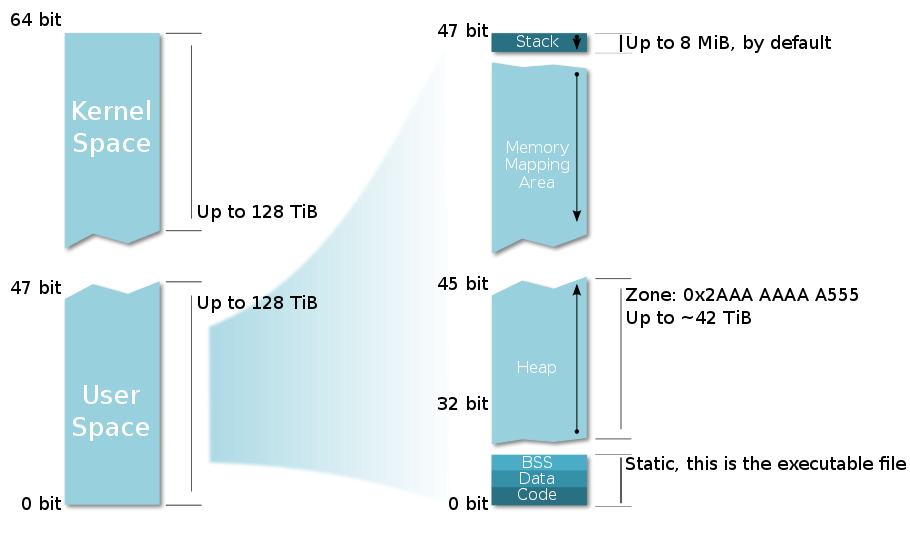
\includegraphics[width=\textwidth]{imgs/memory.png}
		\caption{Linux 64 bit memory management}
		\label{fig:mem}
	\end{figure}
\end{frame}

\begin{frame}{Program Code}
	\begin{block}{Text segment and instruction pointer}
		\begin{itemize}
			\item The code is saved in a RO and executable memory called \emph{Text segment}.
			\item The current instruction is pointed by the \emph{Instruction Pointer}.
			\item The instruction pointer is a value stored into the CPU.
		\end{itemize}
	\end{block}
\end{frame}

\begin{frame}[fragile]{Program Stack}
	\begin{columns}[T]
		\begin{column}{.6\textwidth}
			\begin{itemize}
				\item The stack is where function context, called frame, resides.
				\item The \emph{Base pointer} points to the begin of the frame.
				\item The \emph{Stack  pointer} points to the first available memory location.
			\end{itemize}
			\ccode
			\begin{lstlisting}
				void f() {
				  int xx = 12; int yy = 23;
				  int zz = 24;
				  int sum = xx + yy + zz;
				}
			\end{lstlisting}
		\end{column}
		\begin{column}{.4\textwidth}
			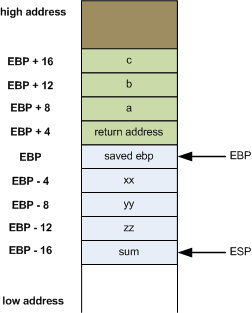
\includegraphics[width=\textwidth]{imgs/stackframe1.png}
			\label{fig:frame1}
		\end{column}
	\end{columns}
\end{frame}
	

\begin{frame}{Assembly Language}
	\subsection{Assembly}
	\begin{block}{Low, low level programming}
		\begin{itemize}
			\item Assembly is the final stage of the programming process.
			\item Each instruction is directly converted into an number.
			\item Writing the number on the CPU Command BUS cause the instruction to
				be executed.
			\item You can access to a set of 64 bit registers:
				\emph{rax, rbx, rcx, rdx, rsi, rdi, r8, r9, r10, r11, r12, r13, r14, r15}
			\item As instruction pointer, base pointer and stack pointer the CPU uses respectively
				\emph{rip, rbp} and \emph{rsp}.
		\end{itemize}
	\end{block}
\end{frame}

\begin{frame}{Assembly Language: function call}
	\begin{block}{The call/ret instructions}
		\begin{description}
			\item[call address]push the RIP into the stack.
			\item[ret]pop the RIP from the stack.
		\end{description}
	\end{block}
	\begin{block}{Creating a frame for the function}
		\begin{itemize}
			\item The callee may need a stack for his own variables.
			\item \emph{RBP} is saved (pushed) into the stack.
			\item The new \emph{RBP} become the old \emph{RSP}.
			\item Before doing ret, the opposite operations must be performed.
		\end{itemize}
	\end{block}
\end{frame}

\begin{frame}{Assembly Language: function call and stack}
	\begin{figure}
		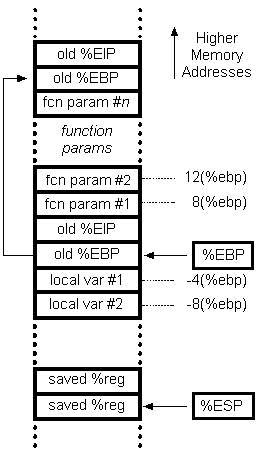
\includegraphics[height=.8\textheight]{imgs/stackframe-cdecl.png}
	\end{figure}
\end{frame}

\begin{frame}{Assembly Language: function call and parameters}
	\begin{block}{Where should I put the parameters?}
		\begin{itemize}
			\item If you are coding in pure ASM, you can do what you want.
			\item Else, you have to follow the conventions (see \url{http://en.wikipedia.org/wiki/X86\_calling\_conventions\#List\_of\_x86\_calling\_conventions}).
		\end{itemize}
	\end{block}
	\begin{block}{Linux calling convention, parameter order}
		First parameters:
		\begin{description}
			\item[x86-64:]rdi, rsi, rdx, rcx, r8, and r9. For system calls, r10 is used instead of rcx.
			\item[IA-32:]ecx, edx. For system calls  ebx, ecx, edx, esi, edi, ebp.
		\end{description}
		Other parameters are pushed into the stack.
	\end{block}
\end{frame}


\begin{frame}{System calls}
	\subsection{Sys-Calls}
	\begin{block}{Invoking the OS}
		\begin{itemize}
			\item User's programs run in the exterior ring with \emph{PL} 3, while
				kernel runs in the inner ring with \emph{PL} 0: Kernel can access to
				the hardware (files, devices, \ldots), user not.
			\item Syscalls form the interface between user and kernel.
			\item E.g.: \emph{open(), read(), write(), chmod(), exec(), \ldots}
		\end{itemize}
	\end{block}
\end{frame}

\begin{frame}[fragile]{Try to use Syscalls}
	\begin{block}{Using assembly}
		\begin{itemize}
			\item In order to ease the programmer duty, syscalls are identified by a
				number.
			\item In modern x86-64 processor, a syscall is invoked using the
				operation \emph{syscall}, putting the id in the register rax.
			\item In modern x86 processor, a syscall is invoked using the
				operation \emph{sysenter} but a lot of operation must be performed
				before, so in the following exercise we will use the old-fashion-way
				\emph{int 80h}, which rises a software interrupt.
		\end{itemize}
	\end{block}
	\acode
	\begin{columns}[T]
		\begin{column}{.4\textwidth}
			\begin{lstlisting}
				mov rdi, 0
				mov rax, 60
				syscall
			\end{lstlisting}
		\end{column}
		\begin{column}{.4\textwidth}
			\begin{lstlisting}
				mov ebx, 0
				mov eax, 1
				int 80h
			\end{lstlisting}
		\end{column}
	\end{columns}
\end{frame}

\begin{frame}[fragile]{Linux Syscalls}
	\begin{block}{Linux}
		\begin{itemize}
			\item Syscalls signatures: \emph{/\ldots{}kernel-sources\ldots/include/linux/syscall.h}
			\item Syscalls numbers: \emph{/usr/include/asm/unistd\_64.h}
		\end{itemize}
	\end{block}
	\acode
	\begin{lstlisting}
		unistd_64.h
		  #define __NR_exit 60
		syscall.h
		  asmlinkage long sys_exit(int error_code);
	\end{lstlisting}
\end{frame}

%%% Shellcode

\section{Writing shellcodes}
\begin{frame}{The final preparation}
	\begin{block}{First steps\ldots}
		\begin{itemize}
			\item Testing platform: \url{http://dl.dropbox.com/u/16169203/data.zip}
			\item Use nasm to compile your assembly code
			\item Feed the tester with the output.
		\end{itemize}
	\end{block}
	\begin{block}{Exercise 0}
		\begin{itemize}
			\item \alert{Create a shellcode that does nothing!}
			\item Test it!
		\end{itemize}
	\end{block}
\end{frame}

\begin{frame}{Using a syscall}
	\subsection{Using a syscall}
	\begin{block}{Exercise 1: The exit syscall}
		\begin{itemize}
			\item \alert{Use the exit syscall to terminate the program}
			\item Change your code setting the return code to $13h$
		\end{itemize}
	\end{block}
\end{frame}

\begin{frame}[fragile,allowframebreaks]{Data reference}
	\subsection{Data references}
	\begin{block}{The reference problem}
		\begin{itemize}
			\item When you write a program you can use global data because, at
				compile time, a static address is associated.
			\item But your shellcode is not compiled with the program it's intended to run.
			\item You must use relative addressing, but before IA-64 it was not possible.
		\end{itemize}
	\end{block}

	\framebreak

	\begin{block}{Old IA-32 way}
		\begin{itemize}
			\item You use a trick: jmp just before the data location, then do a call.
				Et voilà! On the top of the stack there is the data address.
		\end{itemize}
	\end{block}
	\acode
	\begin{lstlisting}
		jmp message
		run:
		  pop ebx ; now ebx contains the string reference
		  ; ... shellcode
		message:
		  call run
		  db 'CeSeNA',0x0a,0
	\end{lstlisting}
	\begin{block}{New IA-64 way}
		\begin{itemize}
			\item IA-64 introduces the RIP relative addressing.
		\end{itemize}
	\end{block}
	\acode
	\begin{lstlisting}
		lea rdi, [rel message] ; now ebx contains
		                       ; the string reference
		; ... shellcode

		message	db 'CeSeNA',0x0a,0
	\end{lstlisting}
	\begin{block}{Generic Way}
		\begin{itemize}
			\item You can pop the string in hex format over the stack.
			\item The stack pointer is then the string reference.
		\end{itemize}
	\end{block}
	\acode
	\begin{lstlisting}
		push 0x000a414e ; 0x00, 0x0a, 'AN'
		push 0x65536543 ; 'eSeC'
		mov ebx, esp ; now ebx contains the string reference
		; ...
	\end{lstlisting}

	\begin{block}{Exercise 2: print on stdout}
		\begin{itemize}
			\item Get the exercise skeleton.
			\item \alert{Understand the code}
			\item Write your own message
		\end{itemize}
	\end{block}

\end{frame}

\begin{frame}[fragile]{Execute a program}
	\subsection{Execute a program}
	\ccode
	\begin{lstlisting}
		unistd_64.h
		  #define __NR_execve 59
		syscall.h
		  int kernel_execve( const char *filename,
		                     const char *const argv[],
		                     const char *const envp[]);
	\end{lstlisting}

	\begin{block}{Exercise 3: A real shellcode, exec a shell!}
		\begin{description}
			\item[4 HaXoRs]
			\item[4 g33k]
			\item[4 n00bz]
		\end{description}
	\end{block}

\end{frame}

\begin{frame}[fragile, allowframebreaks]{Reverse shell}
	\subsection{Reverse shell}
	\ccode
	\begin{block}{One shellcode to rule them all}
		Step to execute:
		\begin{enumerate}
			\item Open a socket to the attacker server.
			\item Duplicate the socket file descriptor into 0 and 1 (and optionally 2).
			\item Exec a shell.
		\end{enumerate}
	\end{block}
	\begin{block}{Step1: Create a socket}
		\begin{itemize}
			\item The standard procedure involves socket creation and connection.
			\item \emph{socket()} and \emph{connect()} syscalls.
			\item The sockaddr\_in structure requires port in network byte order (\emph{htons()}) and ip address in numeric form (\emph{inet\_pton()}).
			\item The usual sockaddr\_in size is 16.
		\end{itemize}
	\end{block}

	\ccode
	\begin{lstlisting}
		long sys_socket(int domain,
		                int type,
                	  int protocol);
		long sys_connect(int fd,
		                 struct sockaddr __user *,
		                 int addrlen);
	\end{lstlisting}

	\ccode
	\begin{lstlisting}
		struct sockaddr_in {
			short            sin_family; // AF_INET
			unsigned short   sin_port; // network order (htons())
			struct in_addr   sin_addr; // As 32 bit
			char             sin_zero[8];
		};
	\end{lstlisting}

	\begin{block}{Step2: Duplicate the file descriptor}
		\begin{itemize}
			\item The return value of socket() is the file descriptor.
			\item The syscall dup2() copy the file descriptor and close the destination.
			\item dup2(fd, 0); dup2(fd, 1), dup2(fd, 2);
		\end{itemize}
	\end{block}

	\ccode
	\begin{lstlisting}
		long sys_dup2(unsigned int oldfd,
		              unsigned int newfd)
	\end{lstlisting}

	\begin{block}{Step3: Exec a shell}
		Already seen ;)
	\end{block}

	\begin{block}{Exercise 4: Reverse shelling}
		Remember to open a server listening into a known address! E.g.: \emph{nc -l
		-p 1234}, preparing reverse shell for 127.0.0.1:1234
		\begin{description}
			\item[4 HaXoRs]
			\item[4 g33k]
			\item[4 n00bz]
		\end{description}
	\end{block}

\end{frame}

\begin{frame}{Shellcode optimization}
	\section{Shellcode Optimization}
	\begin{block}{Why optimization?}
		\begin{itemize}
			\item When writing a shellcode, you must consider various factors. The
				most important are:
				\begin{enumerate}
					\item How the vulnerable program receives the payload.
					\item How long the payload can be.
				\end{enumerate}
			\item The previous exercise solutions, for instance, are not suitable in most cases.
			\item The next slides will discuss about the \emph{NULL} byte presence.
			\item About the payload length, it's all about the exploiter expertise.
		\end{itemize}
	\end{block}
\end{frame}

\begin{frame}[shrink]{String payload}
	\subsection{String payload}
	\begin{block}{zero-bytes problem}
		\begin{itemize}
			\item If the payload is red as a string, C interprets a zero byte as
				string terminator, cutting the shellcode.
			\item Zero-bytes presence is caused by data and addresses:
				\begin{itemize}
					\item \emph{mov rax, 11h} is equivalent to \emph{mov rax, 0000000000000011h}.
					\item \emph{lea rax, [rel message]} is equivalent to \emph{lea rax, [rip + 0000\ldots{}xxh]}.
						\item \emph{execve} for instance, requires a null terminated string and some null parameters.
				\end{itemize}
			\item Solutions are quite straightforward:
				\begin{itemize}
					\item Use \emph{xor} operation to zero a register.
					\item Use when possible smaller part of registers (e.g.: rax $\rightarrow$ eax $\rightarrow$ ax $\rightarrow$ [ah,al])
					\item Use \emph{add} operation: immediate operators are not expanded.
					\item Place not-null marker in strings and substitute them inside the code.
					\item When using relative addressing, place the message above: offset will be negative \cite{mark}.
				\end{itemize}
		\end{itemize}
	\end{block}
\end{frame}

\begin{frame}[fragile, shrink]{Zero-byte removal example}
	\acodenonu
	\begin{columns}[T]
		\begin{column}{.5\textwidth}
			\begin{lstlisting}
				; Set rax = 60h
				xor rax, rax
				mov al, 60
			\end{lstlisting}
			\begin{lstlisting}
				; Set rdi = 12h
				xor rdi, rdi
				add rdi, 12h	
			\end{lstlisting}
			\begin{lstlisting}
				; Negative reference
				message db 'CeSeNA','x'
				lea rdi, [rel message]
			\end{lstlisting}
		\end{column}
		\begin{column}{.5\textwidth}
			\begin{lstlisting}
				; Set to 0 a mem area
				null db 'xxxx'
				xor rbx,rbx
				mov [rel null], ebx
			\end{lstlisting}
			\begin{lstlisting}
				; terminate string with 0
				message db 'CeSeNA','x'
				xor rbx,rbx
				lea rdi, [rel message]
				mov [rdi+7], bl
			\end{lstlisting}
		\end{column}
\end{columns}

\end{frame}
